%This is the first chapter of the dissertation

%The following command starts your chapter. If you want different titles used in your ToC and at the top of the page throughout the chapter, you can specify those values here. Since Columbia doesn't want extra information in the headers and footers, the "Top of Page Title" value won't actually appear.

\chapter[Event Reconstruction][Top of Page Title]{Event Reconstruction}

This chapter describes the reconstruction algorithms used within ATLAS.\todo{cite fermilab lectures}
We will make the distinction between the ``primitive'' objects which are reconstructed from the detector signals from the ``composite'' physics objects we use in measurements and searches for new physics.

\section{Primitive Object Reconstruction}

The primitive objects reconstructed by ATLAS are \textit{tracks} and (calorimeter) \textit{clusters}.
These are reconstructed directly from tracking hits and calorimeter energy deposits into cells.
Tracks can be further divided into inner detector and muon spectrometer tracks.
Calorimeter clusters can be divided into sliding-window clusters and topological clusters (topoclusters).
% \footnotemark
% \footnotetext{Strictly speaking, sliding-window and topological clustering are the names of the algorithms, and thus one could speak of topological electromagnetic clusters or hadronic sliding-window clusters.
% In ATLAS, sliding-window is almost exclusively used to reconstruct electromagnetic objects and topological clustering is almost exclusively used for hadronic clustering, so to avoid confusion we will use this terminology here.
% These choices are entirely based on optimizing the object reconstruction efficiency relative to the fake rate.
% }
\subsection{Inner Detector Tracks}
\todo{cite paper/note}

Inner detector tracks are reconstructed from hits in the inner detector.
These hits indicate that a charged particle has passed through the detector material.
Due to the 2 T solenoid in the inner detector, the hits associated with any individual particle will be curved; this allows one to measure the momentum of the particle.
In any given event, there is upwards of \todo{number}, making it impossible to do any sort of combinatorics to reconstruct tracks\footnotemark.
There are two algorithms used by ATLAS track reconstruction, known as \textit{inside-out} and \textit{outside-in}.

ATLAS first employs the inside-out algorithm.
First, one assumes the track begins at the interaction point.
Moving out from the interaction point, one creates track seeds.
Track seeds are proto-tracks constructed from three hits; these hits can be distributed as three pixel hits, two pixel hits and one SCT hit, or three SCT hits.
One extrapolates the track and uses a combinatorial Kalman filter \todo{cite}, which adds the rest of the pixel and SCT hits to the seeds.
This is done seed by seed, so it avoids the combinatorial complexity involved with checking all hits with all seeds.
At this point, the algorithm applies an additional filter to avoid ambiguities from nearby tracks.
The TRT hits are then added to the seeds in the same procedure; in this way, all hits are associated to a track.

The next step is to figure out the correct kinematics of the track.
This is done by applying a fitting algorithm which outputs the best-fit track parameters by minimizing the track distance from hits, weighted by each hit's resolution.
These parameters are $(d_0, z_0, \eta, \phi, q/p)$ where $d_0$ ($z_0$) is the transverse (longitudinal) impact parameter and $q/p$ is the charge over the track momenta.
This set of parameters uniquely defines the trajectory of the charged particle associated to the track; an illustration of a track with these parameters is shown in Fig.\ref{fig:track_schematic}.

\begin{figure}
\caption{The parameters associated to a track.}
\label{fig:track_schematic}
\includegraphics[width=.45\linewidth]{track_schematic}
\end{figure}

The other track reconstruction algorithm is the outside-in algorithm.
As the name implies, in this case, we start from the outside of the inner detector, in the TRT, and extend the tracks in.
One begins by seeding from TRT hits, and extending the track back towards the center of the detector.
The same fitting procedure is used as in the inside-out algorithm to find the optimal track parameters.
This algorithm is particularly important for finding tracks which originate from interactions with the detector material, especially the SCT.
For tracks from primary vertices, this often finds the same tracks as the inside-out algorithm, providing an important check on the consistency of the tracking procedure.

In the high lumonosity environment of the LHC, even the tracks reconstructed from precision detectors such as those of ATLAS inner detector can sometimes lead to fake tracks from simple combinatoric chance.
Several quality checks are imposed after track fitting which reduce this background.
Seven silicon (pixel + SCT) hits are required for all tracks.
No more than two holes are allowed in the pixel detector; holes are expected measurements from the track that are missing in the pixel detector.
Finally, tracks with poor fit quality, as measured by $\chi^2/ndf$, are also rejected.
Due to the high quality of the silicon measurements in the pixel detector and SCT, these requirements give good track reconstruction efficiency, as seen in Fig.\ref{fig:track_eff} for simulated events\cite{ATL-COM-PHYS-2012-1541}.
\begin{figure}
\caption{Track reconstruction efficiency as a function of track \pt and $\eta$.
The efficiency is defined as the number of reconstructed tracks divided by the number of generate charged particles.} \label{fig:track_eff}
\subfloat[Track reconstruction as a function of \pt.]   {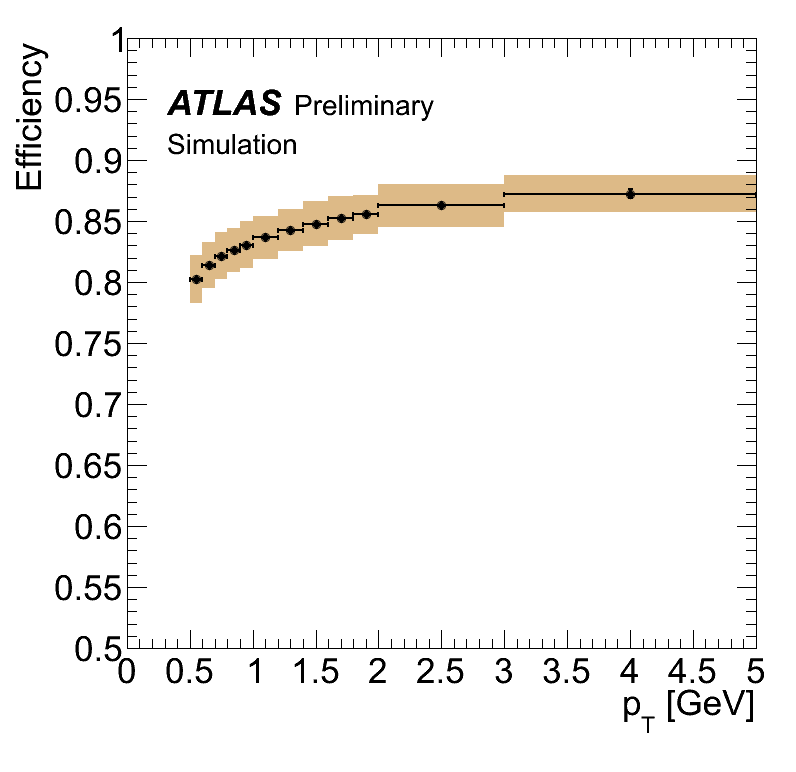
\includegraphics[width=.45\linewidth]{track_eff_pt}}
\subfloat[Track reconstruction as a function of $\eta$.]{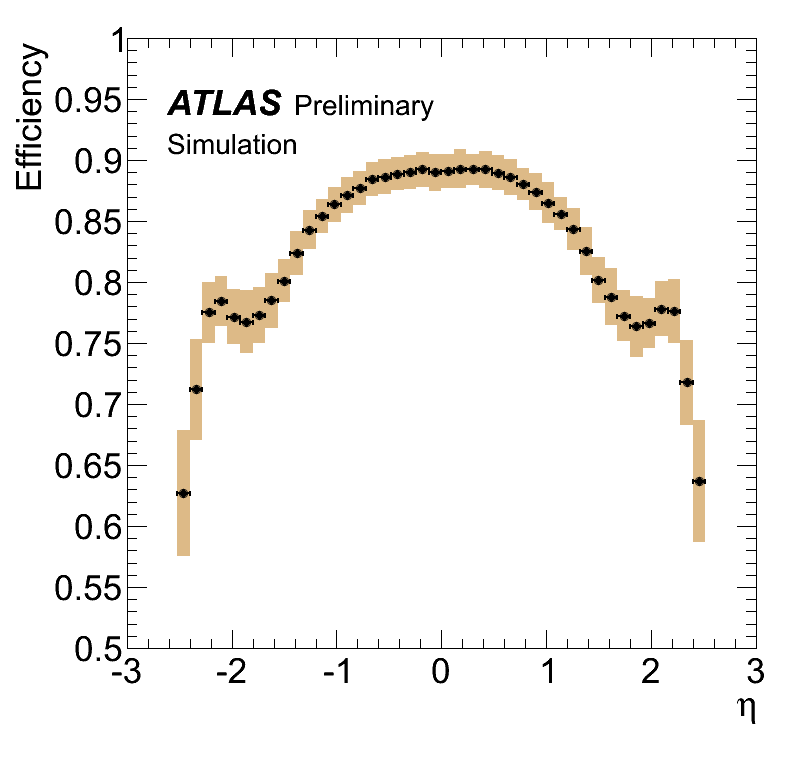
\includegraphics[width=.45\linewidth]{track_eff_eta}} \\
\end{figure}

\subsection{Sliding-window clusters}

The sliding-window algorithm is a way to combine calorimeter cells into composite objects (clusters) to be used as inputs for other algorithms\cite{PERF-2013-03}.
Sliding-window clusters are the primary inputs to electron and photon reconstruction, as described below.
As described in Ch.\ref{ch:atlas}, the electromagnetic calorimeter has high granularity, with a cell size of $(\eta, \phi) = (.025, .025)$ in the coarsest second layer throughout most of the calorimeter.
The ``window'' consists of 3 by 5 cells in the $(\eta, \phi)$ space; all layers are added on this same 2D space.
One translates this window over the space and seeds a cluster whenever the energy sum of the cells is maximized.
If the seed energy is greater than 2.5 \GeV, this seed is called a sliding-window cluster.
This choice was motivated to optimize the reconstruction efficiency of proto-electrons and proto-photons while rejecting fakes from electronic noise and additional particles from pileup vertices.

\subsection{Topological clusters}
\todo{cite paper/note}

Topoclusters are the output of the algorithm used within ATLAS to combine hadronic and electromagnetic calorimeter cells in a way which extracts signal from a background of significant electronic noise\cite{PERF-2014-07}.
They are the primary input to the algorithms which reconstruct jets.

Topological clusters are reconstructed from calorimeter cells in the following way.
First, one maps all cells onto a single $\eta-\phi$ plane so one can speak of \textit{neighboring} cells.
Two cells are considered neighboring if they are in the same layer and directly adjacent, or if they are in adjacent layers and overlap in $\eta-\phi$ space.
The \textit{significance} $\xi_{\text{cell}}$ of a cell during a given event is

\begin{equation}
\calosig = \frac{E_{\text{cell}}}{\sigma_{\text{noise,cell}}}
\end{equation}

where $\sigma_{\text{noise,cell}}$ is measured for each cell in ATLAS and $E_{\text{cell}}$ measures the current energy level of the cell.
One thinks of this as the measurement of the energy \textit{over threshold} for the cell.

Topocluster \textit{seeds} are defined as calorimeter cells which have a significance $\calosig > 4 $.
These are the inputs to the algorithm; one iteratively tests all cells adjacent to these seeds for $\calosig > 2$.
Each cells passing this selection is then added to the topocluster, and the procedure is repeated.
When the algorithm reaches the point where there are no additional adjacent cells with $\calosig > 2$, every positive-energy cell adjacent to the current proto-cluster is added.
This collection of cells is summed; the summed object is known as a topocluster.
An example of this procedure for a simulation dijet event is shown in Fig.\ref{fig:topocluster}.
\begin{figure}
\caption{Example of topoclustering on a simulated dijet event.} \label{fig:topocluster}
\subfloat[All cells with $\calosig > 4$.]{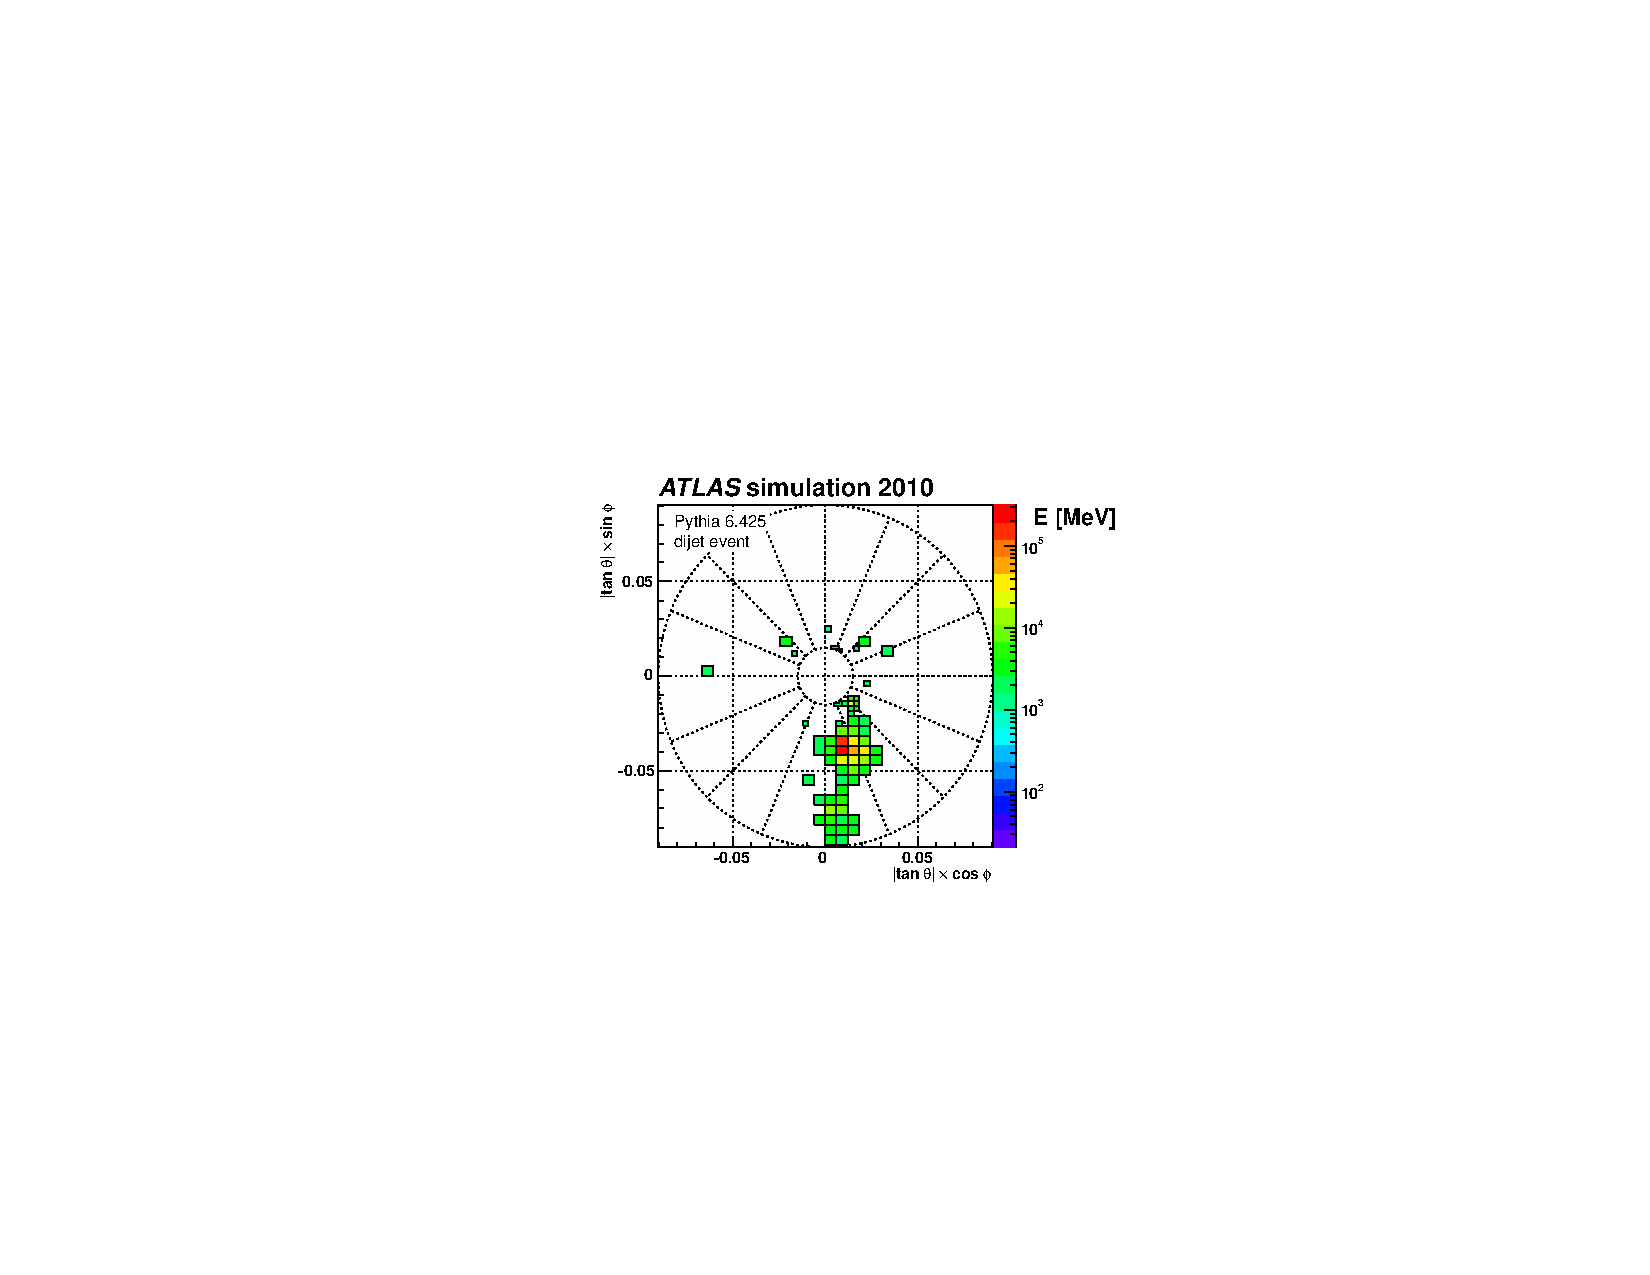
\includegraphics[width=.45\linewidth]{topoclustering_sig4.pdf}}
\subfloat[All cells with $\calosig > 2$.]{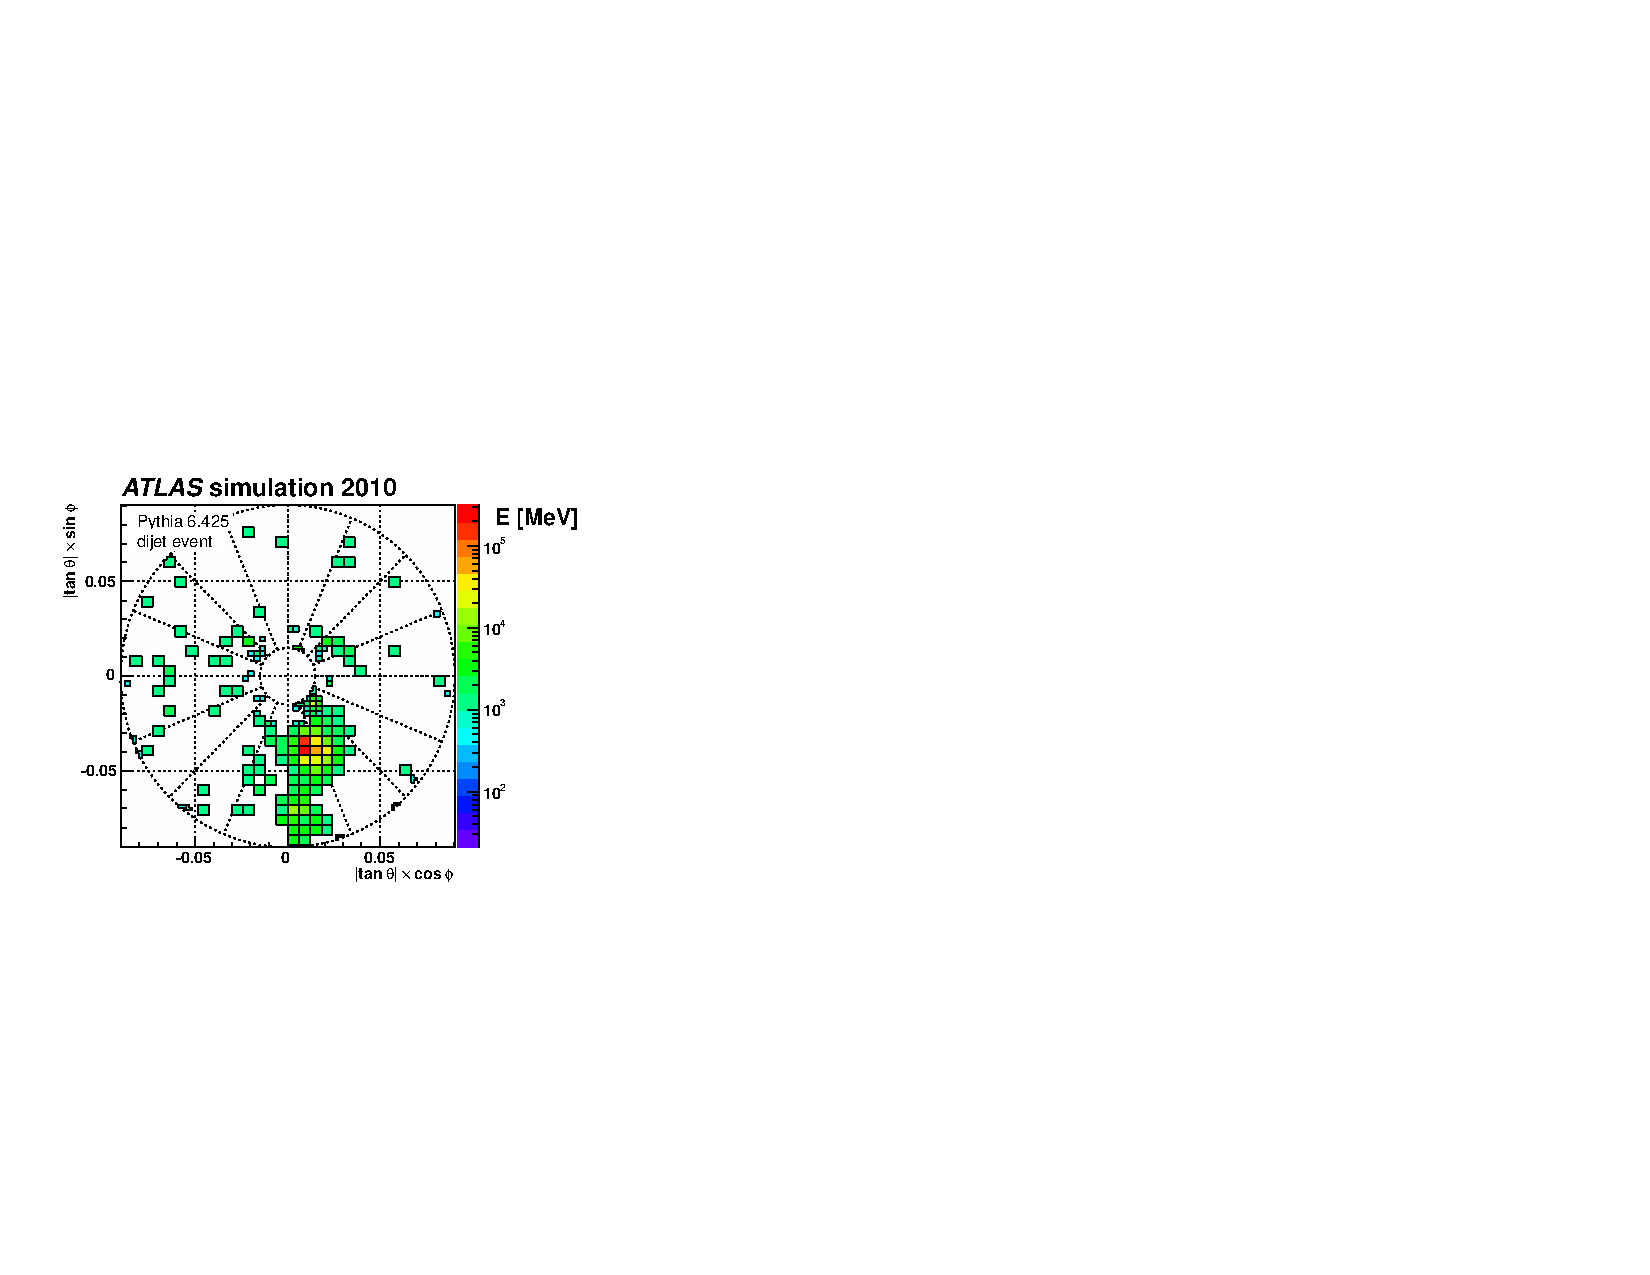
\includegraphics[width=.45\linewidth]{topoclustering_sig2.pdf}} \\
\subfloat[All clustered cells.]{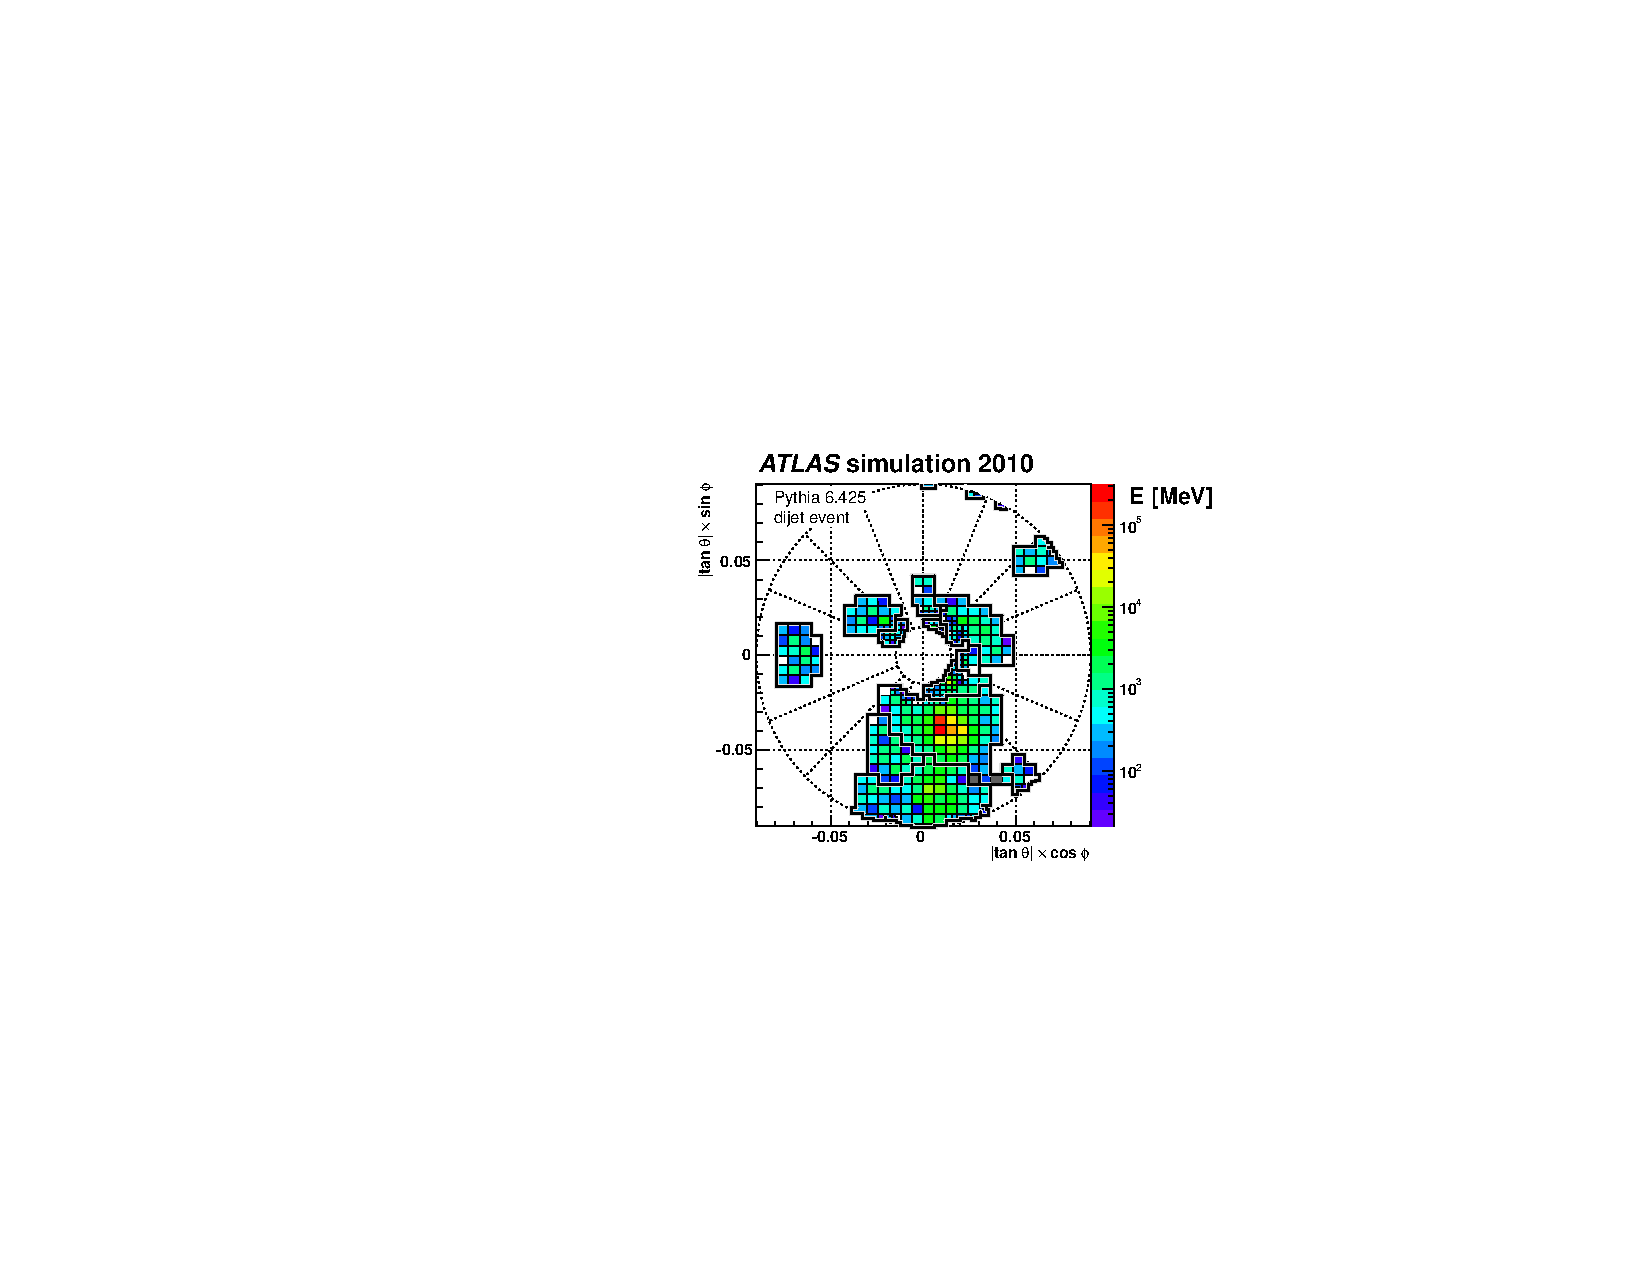
\includegraphics[width=.9\linewidth]{topoclustering_sig0.pdf}}
\end{figure}

\subsection{Muon Spectrometer Tracks}

\section{Physics Object Reconstruction}

There are essentially sixe objects used in ATLAS searches for new physics: electrons, photons, muons, $\tau$-jets, jets, and \met.
The reconstruction of these objects is described here.
A very convenient summary plot is shown in Fig.\ref{fig:atlas_interactions}.
\begin{figure}
\caption{The interactions of particles with the ATLAS detector.
Solid lines indicate the particle is interacting with the detector, while dashed lines are shown where the particle does not interact.} \label{fig:atlas_interactions}
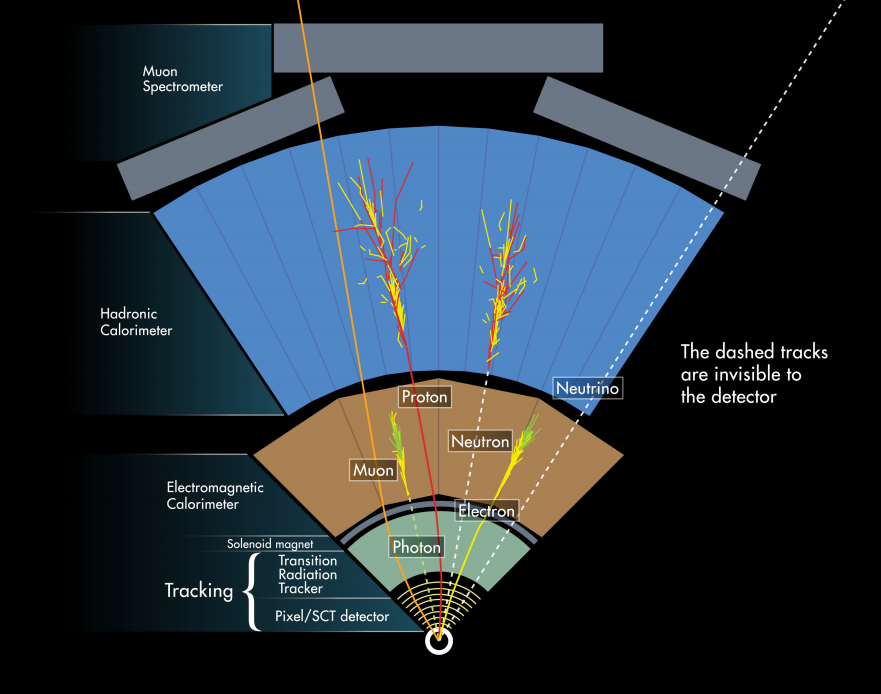
\includegraphics[width=.45\linewidth]{atlas_particle_interactions}
\end{figure}
In this thesis, we present a search for new physics in a zero lepton final state; we will provide additional details about jet and \met reconstruction.
% \subsection{Vertices}

% Vertex reconstruction is an important first step in the reconstruction of ATLAS events\cite{ATL-INDET-PUB-2009-001}.
% If two tracks from charged particles point at the same place inside the detector, we can associate these tracks to that point, which we then call a vertex.
% Generally, we speak of primary vertices associated
% \begin{figure}
% \caption{Depiction of different vertices reconstruct by ATLAS.
% Each ATLAS event has the primary vertex, b-physics vertices, and pileup vertices.} \label{fig:topocluster}
% 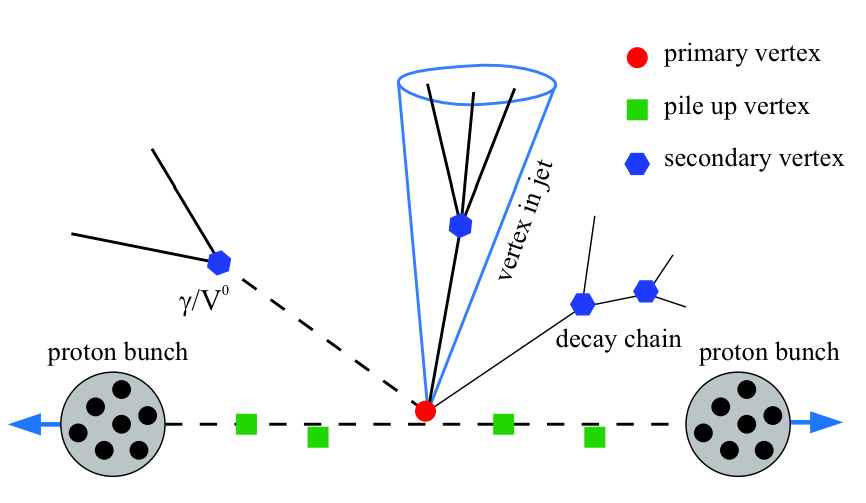
\includegraphics[width=.45\linewdith]{vertex_reconstruction} \\
% \end{figure}

\subsection{Electrons}

Electrons are reconstructed by associating electromagnetic showers in the EM calorimeter with charged particle tracks left in the ID\cite{PERF-2013-03}.
The electromagnetic clusters are reconstructed

\subsection{Photons}
\todo{cite paper/note}

\subsection{Muons}
\todo{cite paper/note}

\subsection{Jets}
\todo{cite paper/note}

\subsection{Missing Transverse Momentum}
\todo{cite paper/notes}

\section{Maybe PFlow?}